% Kompiuterijos katedros šablonas
% Template of Department of Computer Science II
% Versija 1.0 2015 m. kovas [ March, 2015]

\documentclass[a4paper,12pt,fleqn]{article}
\usepackage[unicode,colorlinks=false]{hyperref}


\usepackage[utf8x]{inputenc}
%

\usepackage[L7x]{fontenc}
\usepackage{times}
\usepackage{ucs}

 %package to switch the language
\usepackage{etoolbox}

  %set up of the page margins
\usepackage[top=2cm, bottom=2cm, left=3cm, right=1.5cm]{geometry}

 %1.1 line spacing
\linespread{1.1}


  %page numbering at the right side
\usepackage{fancyhdr}
\pagestyle{fancyplain}
\fancyhf{}
\renewcommand{\headrulewidth}{0pt} 
\fancyhfoffset[RO]{0cm}

  %to number at the bottom (exchange lines to number at the top)
\rfoot{\thepage}
  %\rhead{\thepage} %

% \usepackage[usenames,dvipsnames]{pstricks}
\urlstyle{same}
\hypersetup{
%  citecolor=Blue,
%  linkcolor=Blue,
%  urlcolor=Blue
pdfborder={0 0 0 }
}

 %for includegraphics
\usepackage{graphicx}



\usepackage[toc,page]{appendix}


\usepackage{caption}

 %for source codes
\usepackage{listings}
\lstset{commentstyle=\color{red},xleftmargin=10pt, framexleftmargin=6pt, numbersep=1mm, frame=single, numbers=left,numberstyle=\footnotesize,extendedchars=\true, inputencoding=utf8x,basicstyle=\footnotesize,extendedchars=true,
 keywordstyle=\color{black}\bfseries, breaklines=true, breakautoindent=true,framesep=8pt,linewidth=0.95\textwidth
}

 %for algorithms
\usepackage{algorithm}
\usepackage{algorithmic}
 %instead of the above two packages we can use algorithms2e
 %\usepackage[boxed,linesnumbered,vlined,slide]{algorithm2e}

 %special symbols
\usepackage{amsfonts}
\usepackage{amssymb}
\usepackage{amsmath}

 %for theorem like environments
\usepackage{amsthm}

 \usepackage{datetime}
 \renewcommand{\dateseparator}{--}


% SI system units
\usepackage{siunitx}
\sisetup{detect-all}
% Problem with fonts \SI{x.xx}{\micro\metre}, solved with updmap-sys --enable Map=utm.map
\renewcommand{\sfdefault}{uhv}
\renewcommand{\rmdefault}{utm}
\renewcommand{\ttdefault}{ucr}

% List management (itemize, etc.)
\usepackage{enumitem}

\newcommand*{\urlw}[1]{\href{#1}%
            {\nolinkurl{#1}}}

\numberwithin{equation}{section}


\newtoggle{inLithuanian}
 %If the report is in Lithuanian, it is set to true; otherwise, change to false
\settoggle{inLithuanian}{false}

%create file preface.tex for the preface text
%if preface is needed set to true
\newtoggle{needPreface}
\settoggle{needPreface}{false}

\newtoggle{signaturesOnTitlePage}
\settoggle{signaturesOnTitlePage}{true}


\theoremstyle{definition}
\newtheorem{definition}{\keyWordDefinition}
\newtheorem{example}{\keyWordExample}
\def\QED{\unskip\nobreak\hfill\kern5pt$\Box$}
\def\code#1{\texttt{#1}}

\iftoggle{inLithuanian}{
%\usepackage[L7x]{fontenc}
\usepackage[english,lithuanian]{babel}

\newcommand{\todayiso}{\the\year \dateseparator \twodigit\month \dateseparator \twodigit\day}


\renewcommand{\today}{\number\year\space m. \space \ifcase\month\or
  sausio\or vasario\or kovo\or balandžio\or gegužės\or birželio\or
  liepos\or rugpjūčio\or rugsėjo\or spalio\or lapkričio\or
  gruodžio\fi
  \space\number\day\space d.}


 \usepackage{tocloft}
 \renewcommand\cftsecaftersnum{.} 
 \renewcommand\cftsubsecaftersnum{.} 
 \renewcommand\cftsubsubsecaftersnum{.}

 \usepackage{VUMIFKK}

 \DeclareCaptionLabelFormat{captionlt}{#2 #1}
   %smth is not fine with algorithms 
 \DeclareCaptionLabelFormat{captionltalg}{#2 #1 algoritmas}

 \usepackage{indentfirst}
 \renewcommand{\appendixtocname}{Priedai}
 \renewcommand{\appendixpagename}{Priedai}
 \renewcommand{\contentsname}{Turinys} 

 \renewcommand{\lstlistingname}{išeities kodas}
 \renewcommand{\figurename}{pav}
 \renewcommand{\tablename}{lentelė}


 \captionsetup*[lstlisting]{   
 labelsep=period,labelformat=captionlt
 }
 \captionsetup*[figure]{   
% labelsep=period,
 labelsep=space, %babel redefines pav to pav.
 labelformat=captionlt
 }
 \captionsetup*[table]{   
  labelsep=period,
  labelformat=captionlt
 }
 \renewcommand{\algorithmicrequire}{\textbf{Įvestis:}}
 \renewcommand{\algorithmicensure}{\textbf{Išvestis:}}

 \captionsetup*[algorithm]{   
 labelsep=period,labelformat=captionltalg
 }

\renewcommand{\thmhead}[3]{#2 #1#3}

}
{
%\usepackage[OT1,T1]{fontenc}
%\usepackage[L7x]{fontenc}



\usepackage[english]{babel}
\newcommand{\todayiso}{\twodigit\month \dateseparator \twodigit\day \dateseparator \the\year}
 \captionsetup*[algorithm]{   
 labelsep=period
 }
\captionsetup*[lstlisting]{   
 labelsep=period
 }
 \captionsetup*[figure]{   
 labelsep=period
 }
 \captionsetup*[table]{   
 labelsep=period
 }


}

%some kywords
 \def\keywordAbstract{\iftoggle{inLithuanian}{Santrauka}{Abstract}}
 \def\keywordAbstractOther{\iftoggle{inLithuanian}{Summary}{Santrauka}}
 \def\keyWordIntroduction{\iftoggle{inLithuanian}{Įvadas}{Introduction}}
 \def\keyWordConclusions{\iftoggle{inLithuanian}{Išvados ir rekomendacijos}{Conclusions and Recommendations}}

 \def\keyWordPreface{\iftoggle{inLithuanian}{Pratarmė}{Preface}}
 \def\keyWordAppendice{\iftoggle{inLithuanian}{Priedas}{Appendix}}
 \def\keyWordSignature{\iftoggle{inLithuanian}{parašas}{signature}}
 \def\keyWordDefinition{\iftoggle{inLithuanian}{apibrėžimas}{Definition}}
 \def\keyWordExample{\iftoggle{inLithuanian}{pavyzdys}{Example}}

\newcommand{\bothabstracts}[3]{
\setcounter{secnumdepth}{0}
\newpage
\hspace{2cm}
{\centering{\section{\keywordAbstract}}}

#1
\newpage
\hspace{2cm}
{\centering \section{\keywordAbstractOther}}

\begin{center}{\textbf{#2} }\end{center}

 #3
\setcounter{secnumdepth}{3}
}

 %non-numbered sections: #1 param: for labeling sec:#1, #2 -section title
\newcommand{\sectionWithoutNumber}[2]{\newpage
%\hspace{2cm}
\section*{#1}
\label{sec:#2}
\addcontentsline{toc}{section}{\nameref{sec:#2}}%{#3}
 }



\newcommand{\referenceSources}[1]{
\newpage
\cleardoublepage
\phantomsection
\iftoggle{inLithuanian}{
 \renewcommand{\refname}{Literatūros šaltiniai}

 \addcontentsline{toc}{section}{Literatūros šaltiniai}
 \markboth{\refname}{Literatūros šaltiniai}
 }
{

\addcontentsline{toc}{section}{References}
\markboth{References}{References}
}

\bibliographystyle{plain}
\bibliography{#1}
}



 \newcommand\authorsignature[1]{
\begin{flushright}
 \begin{minipage}[b]{0.45\textwidth}
  \centering
  \rule{\textwidth}{0.5pt}\\
   #1
  \end{minipage}
\end{flushright}
 }




 \newcommand\authorsignatures[5]{%
   \vspace{1cm}
   \authorsignature{#1}
   \ifstrequal{#2}{}{}{\vspace{0.3cm}
     \authorsignature{#2}
     \ifstrequal{#3}{}{}{\vspace{0.3cm}
      \authorsignature{#3}
      \ifstrequal{#4}{}{}{\vspace{0.3cm}
        \authorsignature{#4}
        \ifstrequal{#5}{}{}{\vspace{0.3cm}
         \authorsignature{#5}       
        }
      }
    }
} 
}

\newcommand{\authortitle}{
\iftoggle{signaturesOnTitlePage}{
\tiny{\keyWordSignature}
}{}
}

\newcommand{\depttitlepage}[8]
{
\thispagestyle{empty}
\begin{center}


\includegraphics[width=2cm]{jb_VU_zenklas}

%\vspace{-1cm}

\iftoggle{inLithuanian}
{ 
  VILNIAUS UNIVERSITETAS\\
  MATEMATIKOS IR INFORMATIKOS FAKULTETAS\\
  INFORMATIKOS INSTITUTAS\\
  KOMPIUTERINIO IR DUOMENŲ MODELIAVIMO KATEDRA
}
{
  VILNIUS UNIVERSITY \\
  FACULTY OF MATHEMATICS AND INFORMATICS \\
  INSTITUTE OF COMPUTER SCIENCE\\
  DEPARTMENT OF COMPUTATIONAL AND DATA MODELING
}

\vspace{5cm}

#1\\
\vspace{0.5cm}
\textbf{\Large #2}
\end{center}

\vspace{5cm}


\hspace{0.5\textwidth}
\begin{minipage}{0.4\textwidth}
 \begin{flushleft} 
\iftoggle{inLithuanian}
{
 \ifstrequal{#3}{}{}{Atliko:\\[5pt]}
}
{
\ifstrequal{#3}{}{}{Done by:\\[5pt]}
}

%\noindent
\begin{tabular}{@{}lr}%\setlength\tabcolsep{0pt}
\ifstrequal{#3}{}{}{#3&\hspace{2cm}\authortitle\\[5pt]}
\ifstrequal{#4}{}{}{#4&\authortitle\\[5pt]}
\ifstrequal{#5}{}{}{#5&\authortitle\\[5pt]}
\ifstrequal{#6}{}{}{#6&\authortitle\\[5pt]}
\ifstrequal{#7}{}{}{#7&\authortitle\\}
\end{tabular}

\end{flushleft}

\end{minipage}

\vspace{0.5cm}
\hspace{0.5\textwidth}
\begin{minipage}{0.4\textwidth}
 \begin{flushleft} 

\ifstrequal{#8}{}{}
{

\iftoggle{inLithuanian}
{
Vadovas:
}
{
Supervisor:
}

#8

}

\end{flushleft}

\end{minipage}


\vfill

\begin{center}
Vilnius\\
\the\year
\end{center}

\iftoggle{needPreface}{
 \sectionWithoutNumber{\keyWordPreface}{preface}
Pratarmės (Preface) informacija


\iftoggle{inLithuanian}
{
\vspace{\baselineskip}\hfill
\today
}
{
 \vspace{\baselineskip}\hfill \today
}

 \vspace{5cm}

\iftoggle{signaturesOnTitlePage}{}
{
\authorsignatures{#3}{#4}{#5}{#6}{#7}
}
}{}
\newpage
}


\begin{document}
% #1 -report type, #2 - title, #3-7 students, #8 - supervisor
\depttitlepage{Bachelors Thesis}{Implementation of application for visualization of regularities and randomness in data}{Audrius Baranauskas}
{}{}{}{}% students 2-5
{dr. Tadas Meškauskas}

\tableofcontents


%keywords and notations if needed
\sectionWithoutNumber{Keywords}{keywords}{Pateikiamas terminų sąrašas (jei reikia)}

%both abstracts
\bothabstracts{Santraukos tekstas rašto darbo kalba...}%tex-file of abstract in original language
{Darbo pavadinimas kita kalba} %if work is in LT this title should be in English
{Šio projekto tikslas buvo sukurti interneto aplikaciją, kuri sugebėti sukurti bei kategorizuoti rekurencines diagramas naudojamas duomenų duomenų dėsningumų ir atsitiktinų vizualizavimui.
Aplikacija sugeba reaguoti į varotojo įrenginio dydį.
Dėl šios priežasties ją galima naudotis tiek mobiliuoju telefonu, tiek namų kompiuteriu.
Duomenu kategorizacija yra įgyvendinta panaudojant kovoliucinius neuroninius tinklus.
Neuroninis tinklas gali tiksliai klasifikuoti chaotinius, periodinius bei trendą turinčius duomenis.
Ši publikacija detaliai aprašo aplikacijos vystymo procesą.
Ji taip pat nupasakoja kaip generuojami duomenys kovoliucinio neuroninio tinklo mokymams bei testavimui.
Galiausiai, buvo prieita išvada, kad konvoliucinis neuroninis tinklas gali išmokti kategorizuoti rekurentines diagramas. }%tex-file of abstract in other language


%Introduction section: label is sec:intro
\sectionWithoutNumber{\keyWordIntroduction}{intro}
Įvado tekstas ...


%=============================================================
%========================The main part========================
%=============================================================

\newpage

\section{Signal processing and Recurrence plot}
\label{sec:motivation}
\subsection{Signal processing}

A signal is a function that conveys information about the behaviour of a system
or attributes of some phenomenon \cite{priemer1990introductory}.
For example, measuring the time taken between a weight-driven
pendulum clock's ticks produces signal.
In turn, for the scope of this paper, we defined the term signal processing as
\textit{the science of analyzing time-varying processes} 
\cite{lyons2004understanding}.
By processing a signal we analyzed the non-triviality of a given signal.
Analyzing a signal reveals that some signals 
have properties that can be categorized.

\subsection{Signal property categories}


We have considered the following categories:
\begin{enumerate}
  \item Stationary and non stationary signals
  \item 
\end{enumerate}


Signals have varying properties. Some consist of simple repetitions while others
have no apparent patterns.
For example, measuring the time taken between a weight-driven
pendulum clock's ticks produces a relatively simple (trivial) signal.


\newpage


\section{Web application development}
This project is aimed at creating a web application allowing one to interact with the recurrence plot algorithm in a user friendly manner.
The project offers a feature of classifying data based on the generated plot using convolutional neural networks.
This is an effort to further spread the popularity of this algorithm and help users intuitively grasp how it behaves.


\subsection{Analysis of analogous tools}
As of the date of publishing, only one tool was located capable 
of generating a recurrence plot online \cite{recurrence_plot_tk}. 
There are multiple implementations of the recurrence plot in Python as well as other
languages, but none offer the ability to classify data based on the generated image.

It is noteworthy, that the aforementioned implementations require at least a minimal undertanding of software programming, a computing machine and specific software to compile and run the code. 
This is laborious and is not likely to attract new users to experiment with algorithm.
Based on these factors, a decision was made to create a web based application that requires
as little user knowledge to get started with the algorithm as possible.


%=================================Architecture
\subsection{Architecture}
This project uses the microservices. 
Microservices are small autonomous services deployed independently, with a single and clearly defined purpose \cite{krause2015microservices}. This design approach was chosen due to the flexibility and scalability associated with the architecture. %%%% %%Probably useless sentence
The nature of microservices allows one to easily test, modify or out right replace each one of the components giving more freedom to the developer.
The project ecosystem consists of the following microservices:
\begin{enumerate}
	\item Front end web application
	\item Back end for the web application
	\item Python web server for plotting operations
\end{enumerate}

Communication between microservices is performed via HTTP requests. In general, a query with JSON body is sent to a service and a JSON response along side an image attachment is returned.
Figure~\ref{fig:architecture_diagram} illustrates the microservice architecture of the project and data flow among services.

\begin{figure}[h]
  \centering
  {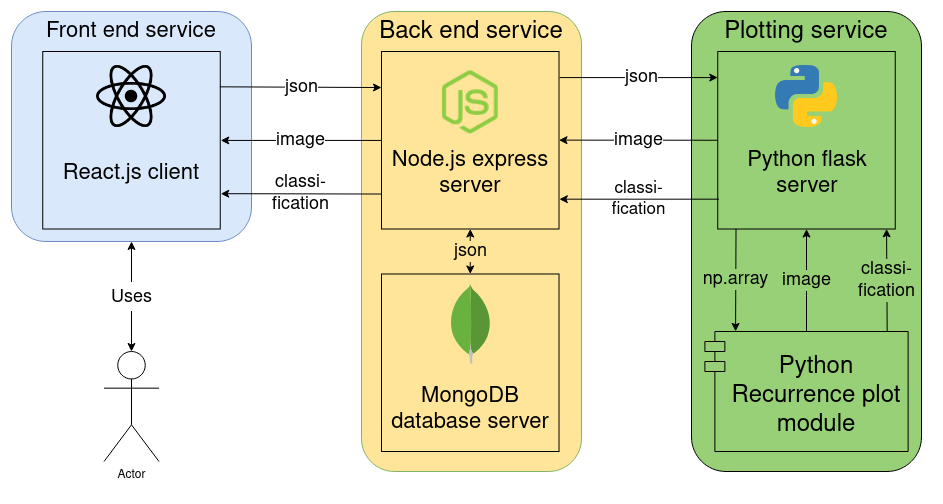
\includegraphics[height=8cm]{assets/architecture_diagram.png}}
  \caption{Microservice architecture structure}
  \label{fig:architecture_diagram}
\end{figure}


%=================================Project structure
\subsubsection{Project structure}
The project is structured so that each microservice resides in an independent directory:
\begin{itemize}
  \item app/
  \begin{itemize}
    \item src/
    \begin{itemize}
      \item components/
    \end{itemize}
    \item public/
  \end{itemize}
  \item server/
  \begin{itemize}
    \item db/
    \item public/
    \item utils/
  \end{itemize}
  \item plotter/
  \begin{itemize}
    \item jupyter/
  \end{itemize} 
\end{itemize}

As the name suggests - \code{/app/} directory contains the front end ReactJS application.
The NodeJS express\cite{express} server resides inside the \code{/server/} directory.
Meanwhile, \code{/plotter/} contains all of the Python source code. That includes the flask \cite{flask} web server, the recurrence plot module, jupyter notebooks for convolutional neural network model development and scripts for model training data generation.


%=================================Project workflow
\subsubsection{Project workflow}
We will now cover an example workflow of the application as per figure~\ref{fig:architecture_diagram}.

When first opening the app, a request is sent to the back end to fetch a list of existing plot data. 
The user selects an entry from the list and fills in remaining parameters for generating a recurrence plot.
A request with select data ID is sent to the back end microservice.
The back end service fetches data from the database and forwards it to the plotting service.
The plotting service generates an image, then runs the image through a convolutional neural network to get classification data.
Finally, the plotting service send the image along with classification data back to the back end service, which in turn forwards it to the front end service.
The front end service displays the image and classification data.


%=================================Microservices
\subsection{Microservices}
The tools used for microservice development were largely open-sourced and relatively modern. 
Front end and Back end services were written in javascript  
based environments - React JS and Node JS respectively.
These choises were made due to the widespread use of javascript in modern web application development providing a large pool of open-sourced libraries and tools.

On the other hand python was the tool used to develop the plotting service. It is known to perform better on data handling and machine learning than javascript alternatives \cite{javascript_vs_python_ml}.
Both Python and Node JS have certain strengths and thus have appropriate community driven libraries and modules to reinforce their leverages in appropriate operations.


%=================================Front end microservice
\subsubsection{Front end microservice}
The front end service is developed using React - A JavaScript library for building user interfaces \cite{react_home}.
SASS is used for styling the apllication due to the intuitive syntax it provides \cite{sass}.
The microservice utilizes the Node Package Manager \cite{npm}.
From the NPM registry, two open sourced libraries are used:
\begin{itemize}
  \item node-fetch - A module that brings window.fetch to Node.js \cite{node-fetch}.
  \item query-string - a tool for building HTTP query string \cite{query-string}.
\end{itemize}
These libraries were used to facilitate communication via HTTP requests with the back end server.

Following the best practices of React development, the app is broken down into reuseable components. 
Figure~\ref{fig:react_component_structure} indicates the application structure denoting components with the standard JSX component notation 
\code{<component />}. We will be using this notation to refeter to JSX components.
\begin{figure}[h]
  \centering
  {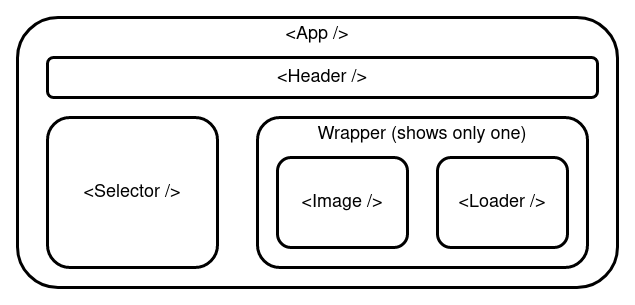
\includegraphics[height=6cm]{assets/react_component_structure.png}}
  \caption{React app component structure}
  \label{fig:react_component_structure}
\end{figure}

Figure~\ref{fig:react_component_structure} indicates that a root \code{<App />} component wraps the whole application.
Initially, only the \code{<Header />}, \code{<Selector />} and \code{<Loader />} components are visible to the user.
The \code{<Selector />} component sends an HTTP GET request to the backend service to retrieve a list of available plot data.
This list is displayed inside the \code{<Selector />} for the user to pick from.
A user must select a data entry and may add optional plotting parameters.
Submitting the \code{<Selector />} form sends an HTTP GET request to the back end service.
The backend service returns a JSON with the location of the generated recurrence plot image and additional parameters.
After handling the server response - the \code{<Loader />} component is replaced by the \code{<Image />}.
During any further plot requests, the \code{<Image />} is briefly replaced by the \code{<Loader />} component to indicate that a request is being processed.


%=================================Back end microservice
\subsubsection{Back end microservice}
The backend microservice also utilizes libraries provided by the Node Package Manager. 
The service runs on an Node JS express server \cite{express}.
The server handles all requests from the front end service.
Server endpoints cover the following operations:
\begin{itemize}
  \item CRUD operations for plot data stored inside the MongoDB database
  \item Requests to generate a recurrence plot using the plotting service
\end{itemize}
The express server communicates with the database server by making use of an open sourced MongoDB object modeling library - mongoose \cite{mongoose}.
The service itself does not generate any plot data, but merely acts as an intermediary between the front end service, the MongoDB database and the plotting service.


%=================================Plotter microservice
\subsubsection{Plotter microservice}
\label{sec:plotter_microservice}
The plotter microservice handles requests to generate and classify recurrence plots. 
The service utilizes numpy\cite{numpy}, scipy\cite{scipy} and matplotlib\cite{matplotlib} open sourced python libraries.

The service consists of 3 main parts:
\begin{enumerate}
  \item Flask - a python web framework
  \item Recurrence plot module
  \item Data classification model
\end{enumerate}
The flask service handles HTTP requests with JSON data as input.
The service processes the input and generates an image using the recurrence plot module.
Image is passed through the convolutional neural network to get the image classification.
An HTTP response is then sent containing the classification data and the generated image as an attachment.


%=================================Recurrence plot module
\subsection{Recurrence plot module}
\label{sec:recurrence_plot_module}
The recurrence plot module is a Python implementation of the algorithm used to generate a recurrence plot.
The module creates a \code{RecurrencePlot} object.
The object takes in several parameters as input allowing one to customize the following features of the generated plot:
\begin{itemize}
  \item D - signal dimension
  \item d - signal delay
  \item compare\_mode - evaluation metric: euclidean and maximum 
  \item target - Prefered pixel percentage of the recurrence plot
  \item deviation - allowed deviation for final pixel percentage
\end{itemize}
As output the module returns the name of the asset in the local storage.
The object can also be manipulated to retrieve various other metrics about the recurrence plot.


%=================================Data classification model
\section{Data classification model}
A recurrence plot reveals certain information about the singal.
After some practice a human can identify whether a given signal exhibits signs of periodity and / or stationarity, has a trend or seems to be random in nature.
The goal of this model is to determine some the aforementioned characteristics of a signal by analyzing the reucrrence plot generated by it.


%=================================Generating training data
\subsection{Generating training data}
It is common knowledge that one requires data to train a convolutional neural network.
The accuracy of a data model heavily weighs on the quality of training data and labeling.
After a brief search for publicly available, labeled and categorized data suitable for training a recurrence plot model, a decision was made for this data to be generated synthetically.


%=================================Training data methodologies
\subsubsection{Training data methodologies}
The source code for generating training assets if written is python programming language.
Open sourced libraries utilized for the creation of assets are listed in section~\ref{sec:plotter_microservice}.
All of the following signals and their graphs are generated by utilizing
the aforementioned libraries and the recurrence plot module.
For every signal a complementary graph image is generated to help visualise the data which resulted in the recurrence plot.
Due to the module flexibility every chaotic and periodic asset had randomised values for D - Dimension and d - delay.
In addition, most aspects of each graph had a randomised flaoting point number be added or subtracter.
This aided in generating a more diverse set of training assets.
The number of assets chosen was arbitraty - 1000 sygnals for each training label.
That amounts to a total of 3000 recurrence plot images used for training the CNN.
The source code for generating assets and associated graphs is inside the \code{/plotter/generate-cnn-assets.py} file.


%=================================Choosing classification features
\subsubsection{Choosing classification features}
Before generating the data it is important to recognize what the convolutional neural network is expected to learn from it.
The \emph{what can it learn?} aspect of a CNN is mostly limited by the labeled data we can provide.
A choise was made to classify plot images into one of the three groups:
\begin{itemize}
  \item Plotted signal is chaotic
  \item Plotted signal has a trend
  \item Plotted signal has is periodic
\end{itemize}
We will explore the reasoning of this decision by exploring the limitations of generating labeled signals.


%=================================Chaotic signal
\subsubsection{Chaotic signal}
A relatively simple signal to identify is a chaotic signal.
Chaotic, means it has no distinguishable pattern - random.
This signal can be generated rather easily - by calling a random number generator for each entry in the signal.
It is also advantageous, that chaotic signal does not trigger any other feature attribute except for stationarity.
A chaotic signal tends to have a high level of stationary meaning it is dispersed fairly evenly across the recurrence plot.
Figure~\ref{fig:generated_chaotic} displays a signal (a) and the generated recurrence plot (b) from the training set.
This signal is labeled as chaotic and is one of the signals used for training the convolutional neural network.


\begin{figure}
  \centering
  \subfloat[\centering Chaotic signal]{{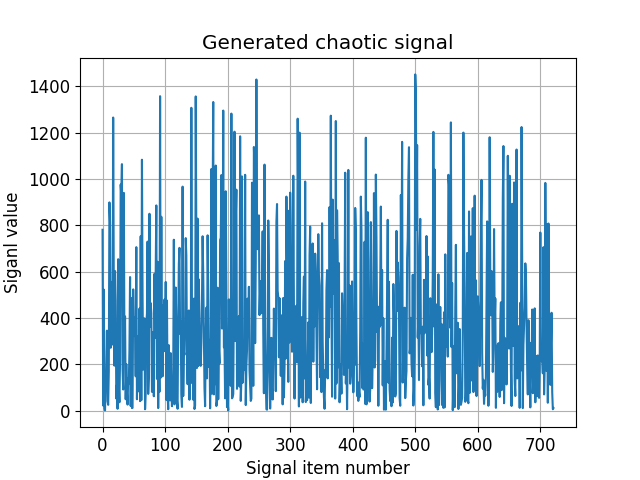
\includegraphics[height=5.5cm]{assets/chaos_graph.png} }}
  \qquad
  \subfloat[\centering Recurrence plot. Pixel target=17.5\%, D=2, d=1]{{
\includegraphics[height=5cm]{assets/chaos_rp.png} }}
  \caption{Chaotic signal and recurrence plot generated by it}
  \label{fig:generated_chaotic}
\end{figure}


%=================================Periodic signal
\subsubsection{Periodic signal}
For a human, identifying a signal with a periodic characteristic is not too strenuous either.
Unfortunately we cannot consider the periodicity of a signal without considering the stationarity of it.
Stationarity is generally observed by the homogeneity of a signal.
In layman terms - how evenly the pixels are spread across the recurrence plot.
Looking back at figure~\ref{fig:generated_chaotic} we can see that a chaotic signal is highly stationary as the pixels are spread fairly evenly.
Figure~\ref{fig:generated_periodic_sin} illustrates a signal (a) from the periodic training set and the recurrence plot (b) that is generated from it.
We can see that this siganl forms a grid pattern.
The pattern stretches across the whole image therefore this signal is also stationary.
It would be difficult to generate periodic data that is not stationary, but the same applies to chaotic data.
This is the reason why stationarity is not one of the attributes measured by the model.
Determining the level of periodicity is beyond the scope of this particular neural netowrk.
\begin{figure}
  \centering
  \subfloat[\centering Sine wave signal]{{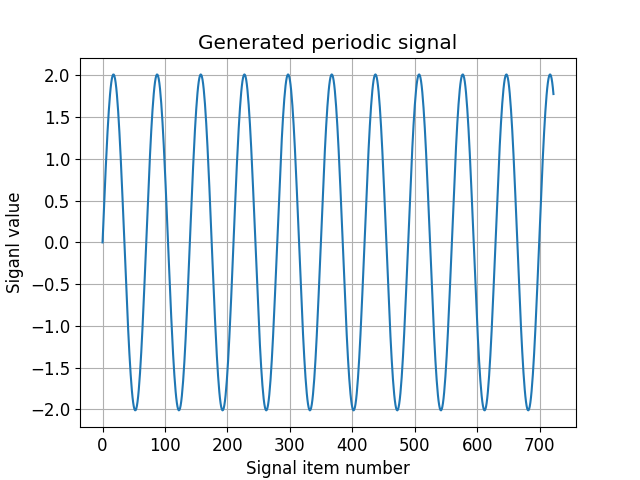
\includegraphics[height=5.5cm]{assets/period_graph_sin.png} }}
  \qquad
  \subfloat[\centering Recurrence plot. Pixel target=17.5\%, D=3, d=2]{{
\includegraphics[height=5cm]{assets/period_rp_sin.png} }}
  \caption{Periodic sine wave form signal and recurrence plot generated by it}
  \label{fig:generated_periodic_sin}
\end{figure}

A periodic signal wave can have difference forms.
The signal in figure~\ref{fig:generated_periodic_sin} is generated from a sine wave.
To provide the model with more diverse training data - two additional distinct wave functions were used to generate the training data.
Figure~\ref{fig:generated_periodic_square} illustrates a signal with a square wave. See the signal wave (a) on the left and generated recurrence plot on the right (b).
\begin{figure}
  \centering
  \subfloat[\centering Square wave signal]{{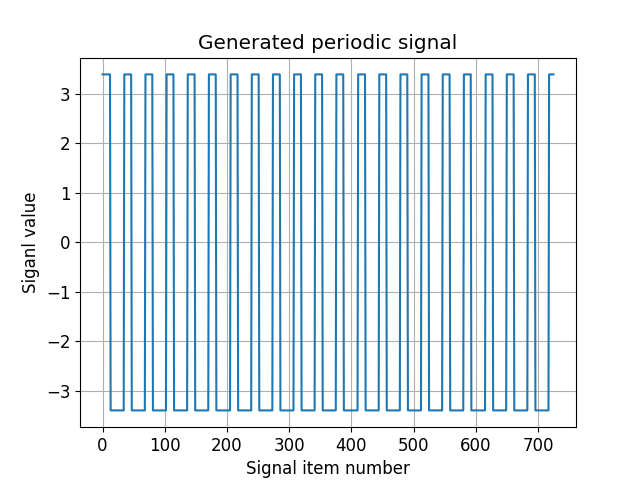
\includegraphics[height=5.5cm]{assets/period_graph_square.png} }}
  \qquad
  \subfloat[\centering Recurrence plot. Pixel target=17.5\%, D=4, d=2]{{
\includegraphics[height=5cm]{assets/period_rp_square.png} }}
  \caption{Periodic square wave form signal and recurrence plot generated by it}
  \label{fig:generated_periodic_square}
\end{figure}
The final waveform to be used for periodic images is the sawtooth waveform.
Figure~\ref{fig:generated_periodic_sawtooth} illustrates the wave signal (a) and the recurrence plot generated (b) using it.

\begin{figure}
  \centering
  \subfloat[\centering Sawtooth wave signal]{{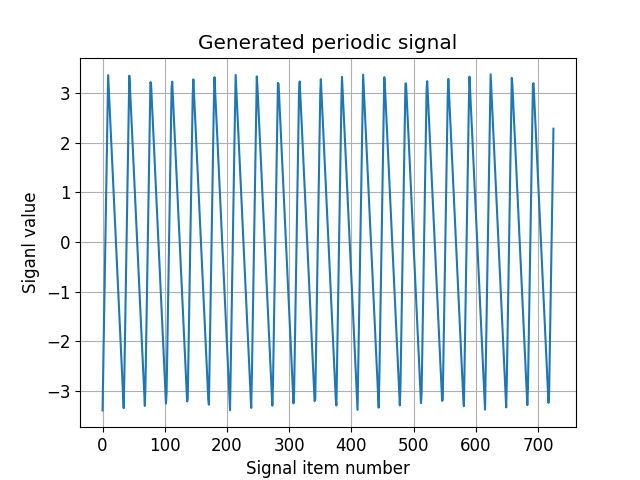
\includegraphics[height=5.5cm]{assets/period_graph_sawtooth.png} }}
  \qquad
  \subfloat[\centering Recurrence plot. Pixel target=17.5\%, D=4, d=2]{{
\includegraphics[height=5cm]{assets/period_rp_sawtooth.png} }}
  \caption{Periodic sawtooth wave form signal and recurrence plot generated by it}
  \label{fig:generated_periodic_sawtooth}
\end{figure}


%=================================Signal with a trend
\subsubsection{Signal with a trend}
A trend signal is quite distinguishable by it's tendency to be less stationary than the previous two.
Recurrence plot of a non synthetic trend signal appears to center aruond the diagonal simetry line and tends to have an increasing width towards either side of the image.
Figure~\ref{fig:generated_trend} illustrates an example trend signal (a) and the recurrence plot generated using it (b).
This is one of the labeled samples used in training the convolutional neural netowrk.

These signals are generated by using a randomly generated data starting point. Then generating an integer within a given range to simulate increasing or decreasing data.
Finally slightly increasing the average signal value by a flat value multiplied by an exponent.
This allows synthetic trend data to either increase linearly or exponentially.
Looking closely to figure~\ref{fig:generated_trend} image on the left we can see that the trend data exhibits an exponentially increasing in values.
The exponent is picked to be small so that the synthetic signal appears more 
natural.

\begin{figure}
  \centering
  \subfloat[\centering Trend signal]{{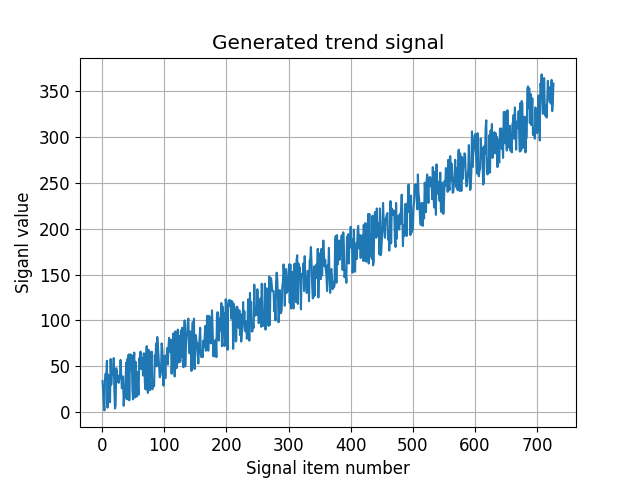
\includegraphics[height=5.5cm]{assets/trend_graph.png} }}
  \qquad
  \subfloat[\centering Recurrence plot. Pixel target=17.5\%, D=4, d=2]{{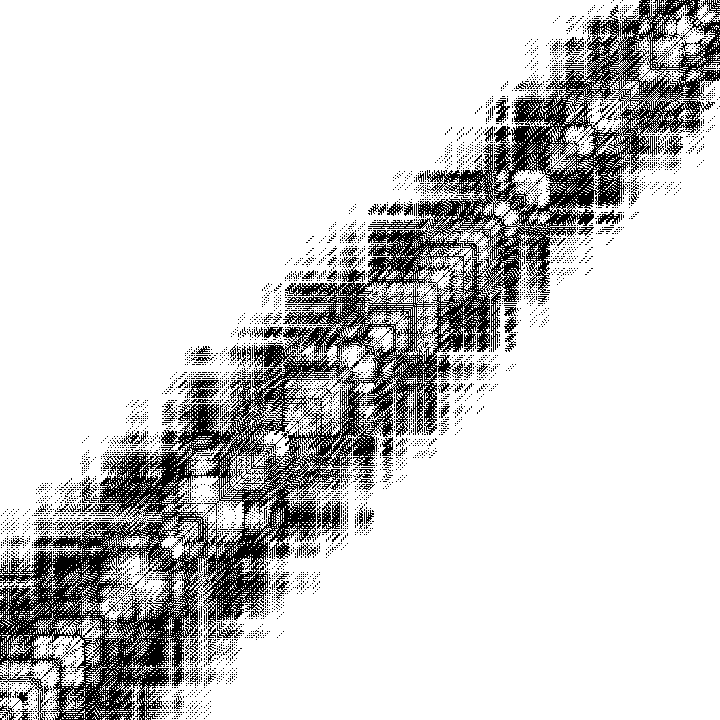
\includegraphics[height=5cm]{assets/trend_rp.png} }}
  \caption{Trend signal and recurrence plot generated by it}
  \label{fig:generated_trend}
\end{figure}

\subsection{Data processing}


% \begin{figure}[h]
%   \centering
%   {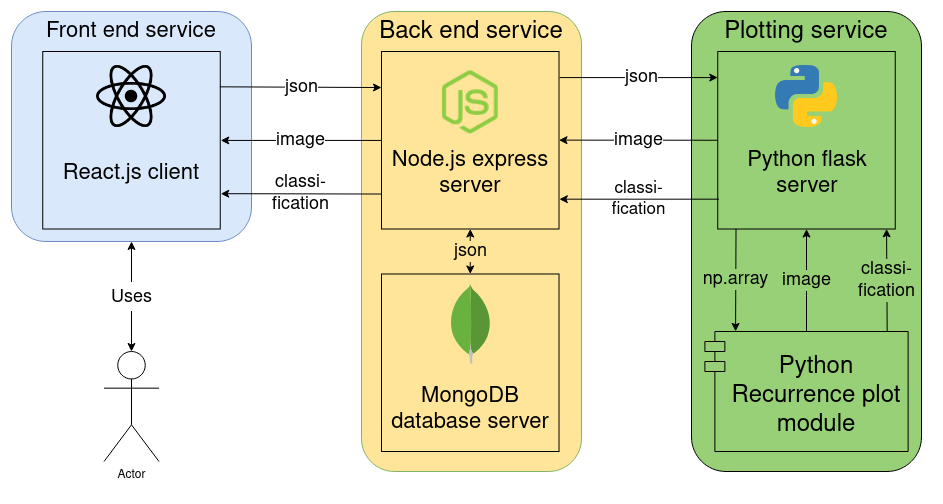
\includegraphics[height=8cm]{assets/architecture_diagram.png}}
%   \caption{Microservice architecture structure}
%   \label{fig:architecture_diagram}
% \end{figure}

% Identify what are the attributes 

% An ideal training dataset would have a sizeable amount CNN
% In order for a 
% This decision was based purely on the ability to generate data that is labeled accordingly.


% \subsection{Model limitations}
%We will go more in depth about each microservice in later sections.


% For the scope of this paper, we defined the term signal 
% processing as \textit{the science of analyzing time-varying 
% processes} \cite{lyons2004understanding}.




% \subsection{Signal classification}
% Signals have several classes. For the scope of this paper we considered
% the classes \cite{lathi1998signal}:
% \begin{enumerate}
%   \item Stationary and non-stationary signals
%   \item 
%   \item Periodic, quasi periodic and aperiodic signals 


% \end{enumerate}






% Some signals are inherently simple such as the time taken
% a falling object or

% \begin{lstlisting}
%   sygnalStates = []

%   # Generate data pairs, tripplets, quadruplets... D - plets
%   for i in range(0, self.M):
%       state = []

%       for j in range(0, self.D):
%           state.append(self.data[i+(j*self.d)])

%       sygnalStates.append(state)
% \end{lstlisting}



% \newpage
% \section{Pirmasis skyrius}
% \label{sec:motivation}

% asa \cite{recurrence-plot}



% \subsection{Pirmojo skyriaus poskyris}
% \label{sec:example}
% Pateikiamas \ref{sec:example} poskyrio tekstas. Vienas iš šaltinių~\cite{KTZ}. Visas ~\cite{KTV} turinys priklauso \ref{sec:motivation} skyriui.

% \subsubsection{Pirmojo skyriaus pirmo poskyrio poskyris}
% \label{sec:data}
% Pateikiamas trečio lygio poskyrio tekstas.

% \begin{equation}
%   x = \sum_{i=1}^N m_i
% \end{equation}

% \begin{table}[!ht]\centering
%   \caption{Lentelė ... }
%   \label{tabl:table}
%   \begin{tabular}{l|r|}
%     test & test \\ \hline
%     test & test \\
%   \end{tabular}
% \end{table}

% Sprendimas pristatomas \ref{alg:1} algoritme, o įgyvendinimas -- \ref{abc} išeities kode.

% \begin{algorithm}\caption{Algoritmas uždavinio sprendimui}
%   \label{alg:1}
%   \begin{algorithmic}
%     \REQUIRE
%     \ENSURE
%     \STATE a \AND b
%   \end{algorithmic}


% \end{algorithm}



% \begin{lstlisting}[caption={Pagrindinio metodo žingsniai},label={abc}]
% public static void main(String args[]){
% }
% \end{lstlisting}

%Conclusions section
\newpage
\sectionWithoutNumber{\keyWordConclusions}{conclu}
During the research and development phases of this project, the following goals were achieved:
\begin{itemize}
    \item The recurrence plot was analysed to evaluate what can be determinen from the visualization. Several observable characteristics were distinguished. A local implementation of the recurrence plot was developed and utilized throughout the application.
    \item A convolutional neural network, capable of identifying the characteristics of a recurrence plot, was developed and trained. The trained data model performed with high accuracy.
    \item An web application for generating recurrence plots was developed. A microservice architecture was used develop the application providing a modern, scalable solution. The application utilizes the aforementioned CNN to provide information about the generated, that a novel user might not distinguish.
\end{itemize}

The application functionality can be yet improved. Microservice could be containerized to provide easier deployment. The front end part of the application could support full CRUD operations for managing of data in the database. So far this this can only be done by accessing the backend service via an exposed API.

%ateities darbų gairės, planas/next steps of the work
\sectionWithoutNumber{Ateities tyrimų planas}{future}{Pristatomi ateities darbai ir/ar jų planas, gairės tolimesniems darbams....}


%file literatureSources.bib
\referenceSources{literatureSources}



%% this part is optional
\newpage
\begin{appendices}
  Dokumentą sudaro du priedai: \ref{app:a} priede  ....
  \newpage
  \section{Pirmojo priedo pavadinimas}
  \label{app:a}
  Pirmojo priedo tekstas ...

  \newpage
  \section{Antrojo priedo pavadinimas}
  Antrojo priedo tekstas ...

\end{appendices}


\end{document}
